% ===================================================================================================
\chapter{Results}
% ===================================================================================================

% ----------------------------------------------------------------------------------
\section{Vacancies}
% ----------------------------------------------------------------------------------
In fig. (\ref{Fig:1Vac_results}) we can see the number of T and H atoms bound to the monovacany as a function of time, for three different temperatures. 
For comparison, simulations without any added H atoms were run with tritium being removed purely due to diffusion. 

\begin{figure}[ht]
\begin{subfigure}{.5\textwidth}
  \centering
  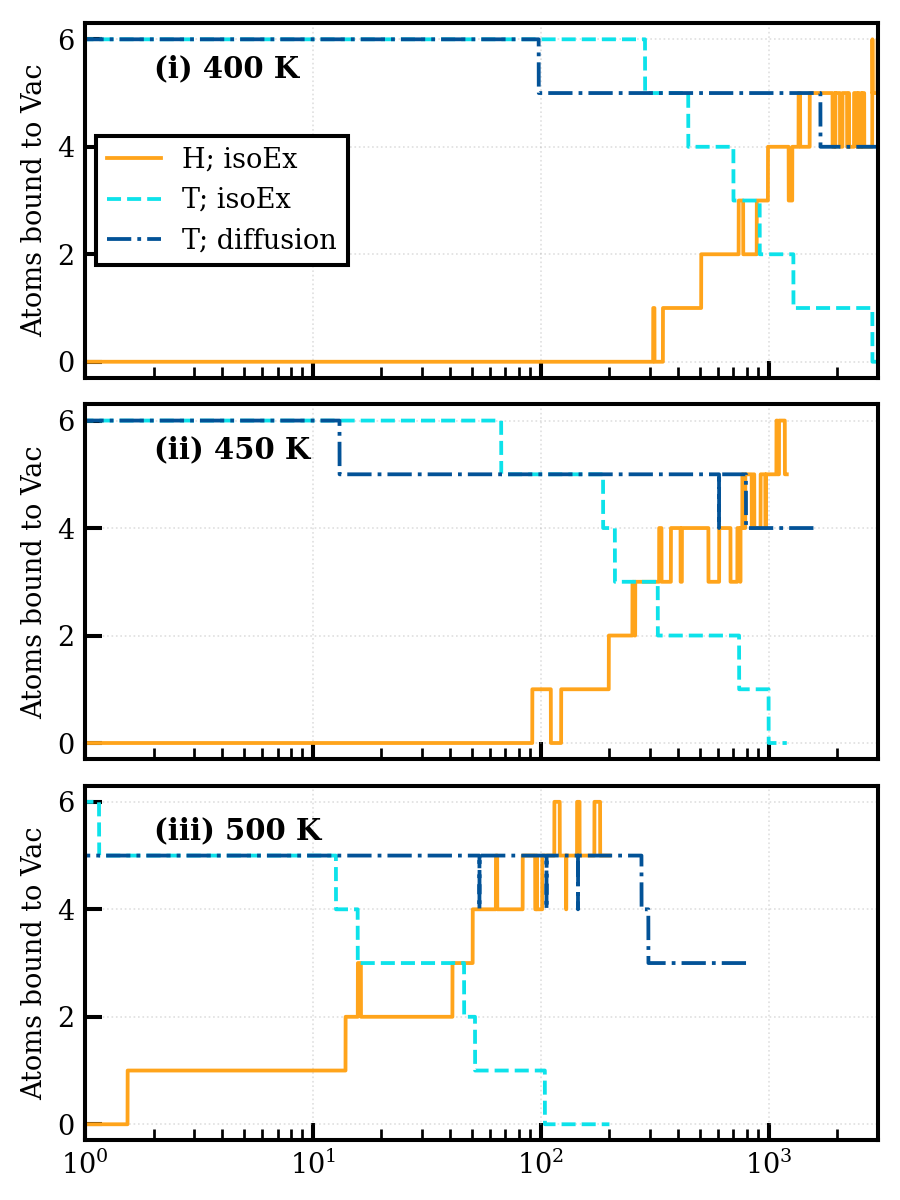
\includegraphics[width=0.99\textwidth]{1Vac_isoEx_HT_log.png}  
  \caption{Logarithmic time scale}
  %\label{fig:sub-first}
\end{subfigure}
\begin{subfigure}{.5\textwidth}
  \centering
  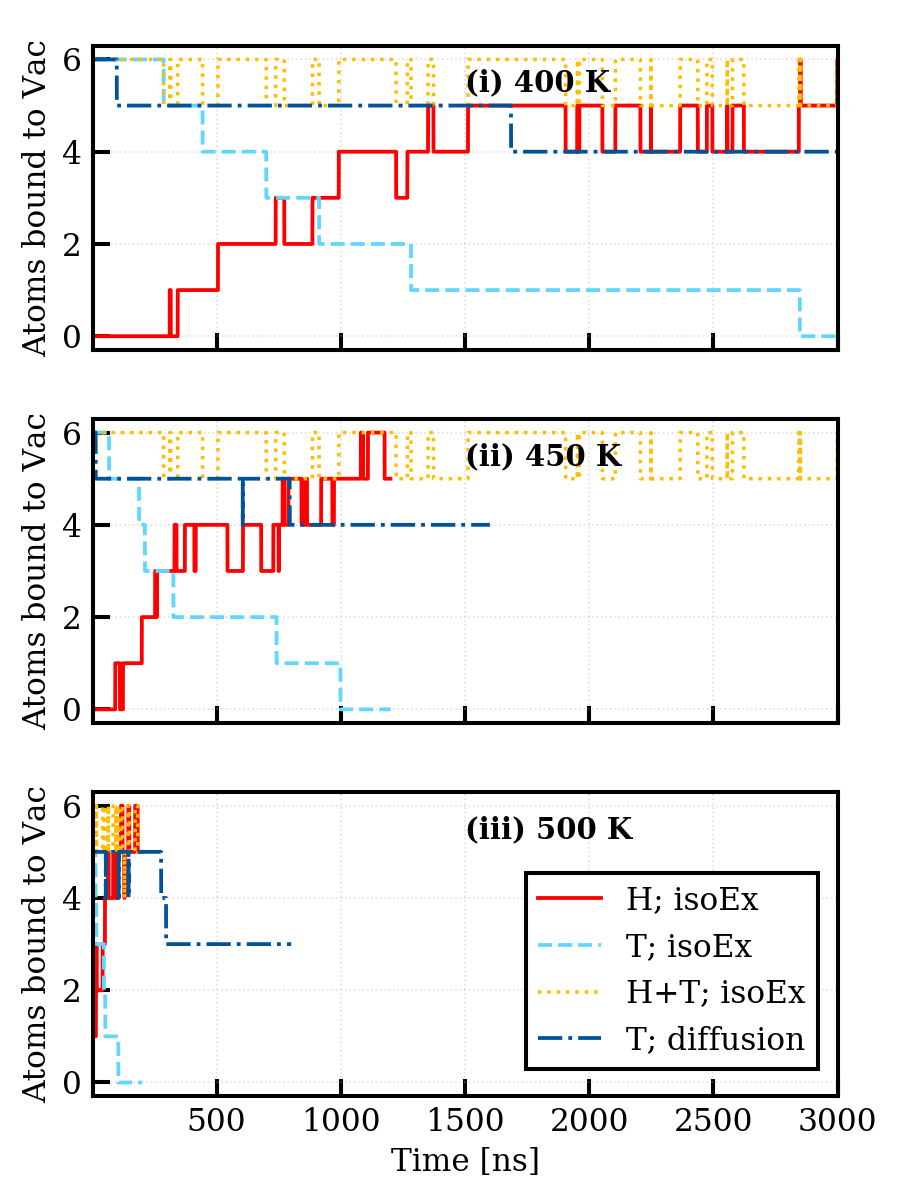
\includegraphics[width=0.99\textwidth]{1Vac_isoEx_HT.png}  
  \caption{Linear time scale}
  %\label{fig:sub-second}
\end{subfigure}
\caption{Number of H and T atoms in the monovacany for isotope exchange and diffusion simulations}
 \label{Fig:1Vac_results} 
\end{figure}


\begin{figure}[ht]
\begin{subfigure}{.5\textwidth}
  \centering
 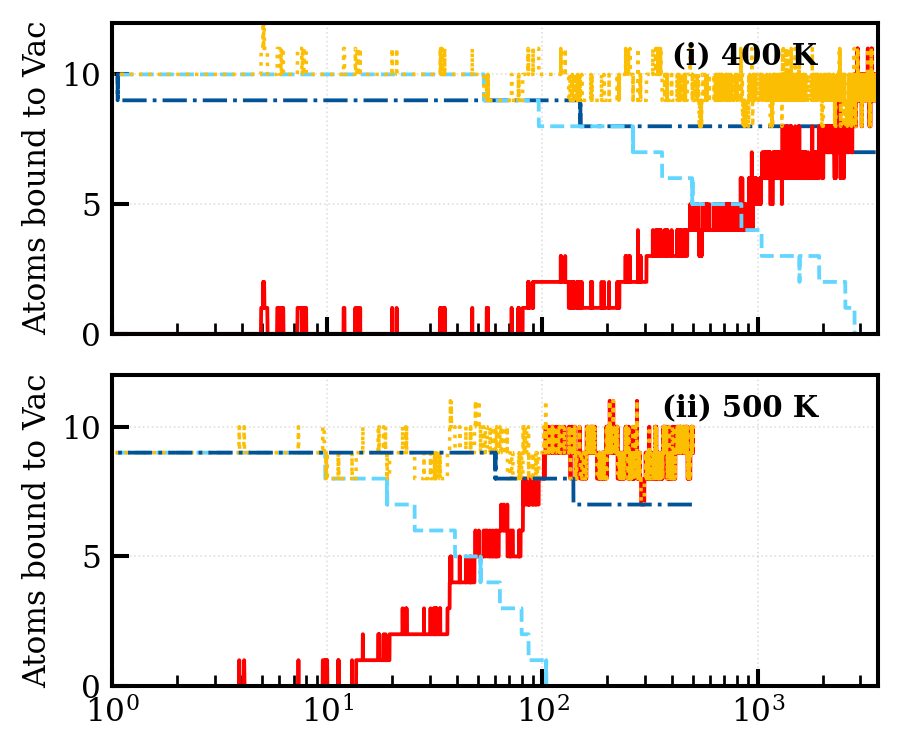
\includegraphics[width=0.99\textwidth]{2Vac_isoEx_HT_log.png}  
  \caption{Logarithmic time scale}
  %\label{fig:sub-first}
\end{subfigure}
\begin{subfigure}{.5\textwidth}
  \centering
  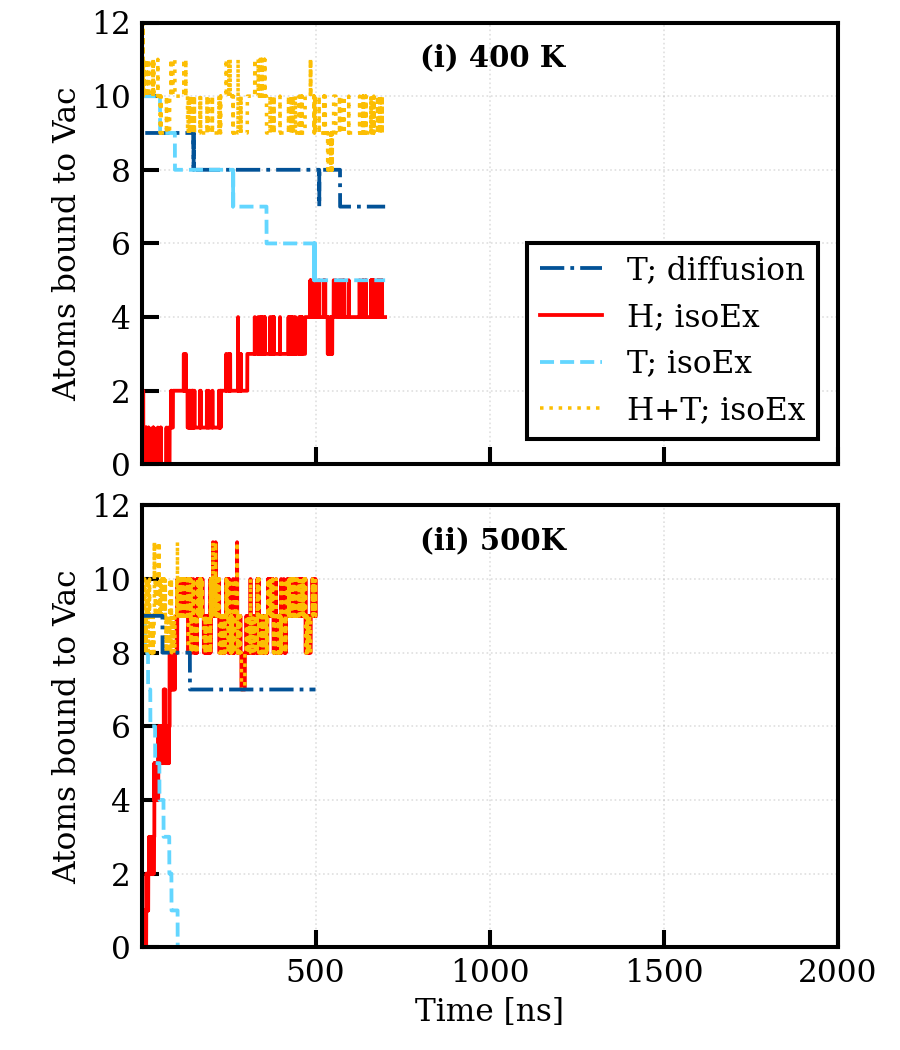
\includegraphics[width=0.99\textwidth]{2Vac_isoEx_HT.png}  
  \caption{Linear time scale}
  %\label{fig:sub-second}
\end{subfigure}
   \caption{Number of H and T atoms in the divacany for isotope exchange and diffusion simulations}
   \label{Fig:2Vac_results} 
\end{figure}

From the figures \ref{Fig:1Vac_results} and \ref{Fig:2Vac_results} it is evident that the addition of T significantly increases the rate of T removal from both mono- and divacancies. 

Because of the H atoms being lighter, and thus being slightly more mobile than T, one would assume H to leave the monovacancy at a faster rate than T. 
This is exactly what can be seen when running a simulation with the hydrogen isotopes inverted i.e. having six H atoms initially bound to the vacancy and surrounded by 20 uniformly distributed T atoms. 
In this inverted setting, (Fig. \ref{Fig:1Vac_results}; subfigs. a.iv and b.iv) the complete isotope exchange at the vacancy can be seen to occur in just over 200 ns, compared to the 500 ns required to replace T with H in our earlier simulation.  

Although to the potential gives smaller binding energy values for the hydrogen-vacancy interaction than DFT (Fig. \ref{Fig:Ebind1H_DFT}), the comparison simulations with only tritium and no added H (Fig. \ref{Fig:1Vac_results}) clearly show that qualitative results are still valid.

\begin{figure}[!ht]
\center
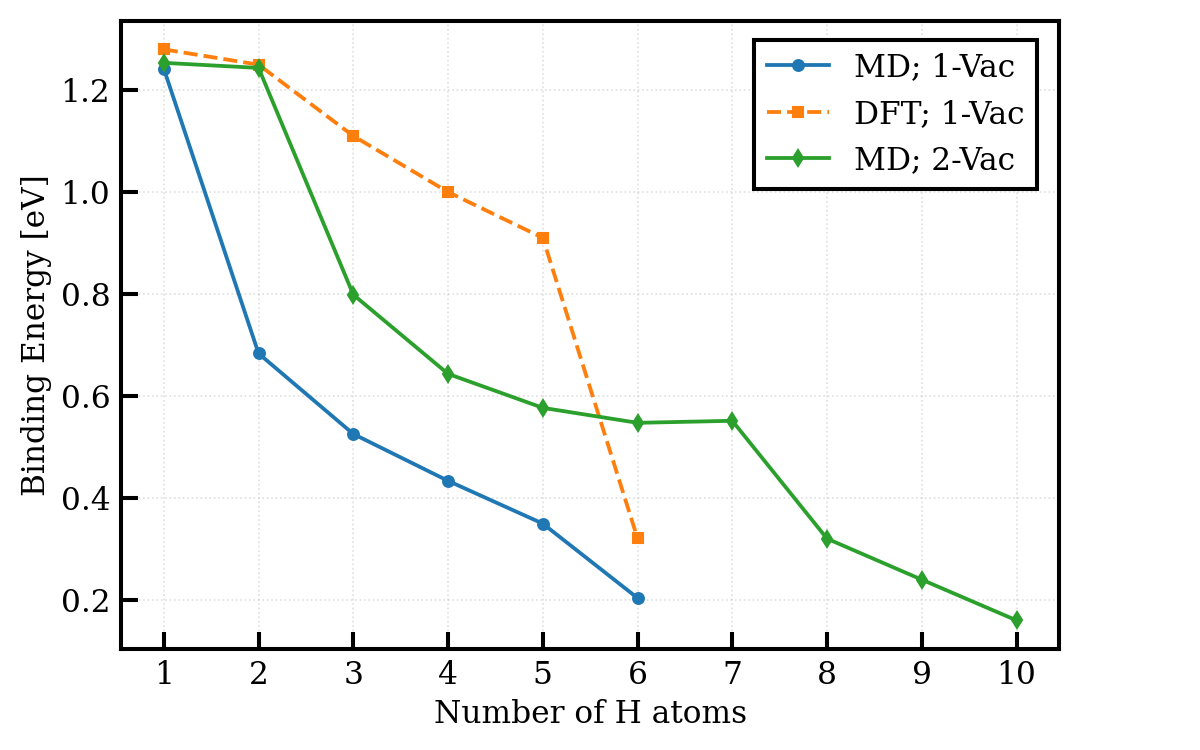
\includegraphics[width=0.6\linewidth]{Ebind.png}
\caption{Comparision of the H-W binding energy in EAM1 by Bonny \textit{et. al} and DFT results by Heinola \textit{et. al. }\cite{heinolaTungstenDFT}}
\label{Fig:Ebind1H_DFT}
\end{figure}




% ----------------------------------------------------------------------------------
\section{Dislocations}
% ----------------------------------------------------------------------------------
The dislocation results are shown in fig. \ref{Fig:disloc_results}

\begin{figure}[ht]
\begin{subfigure}{.5\textwidth}
  \centering
 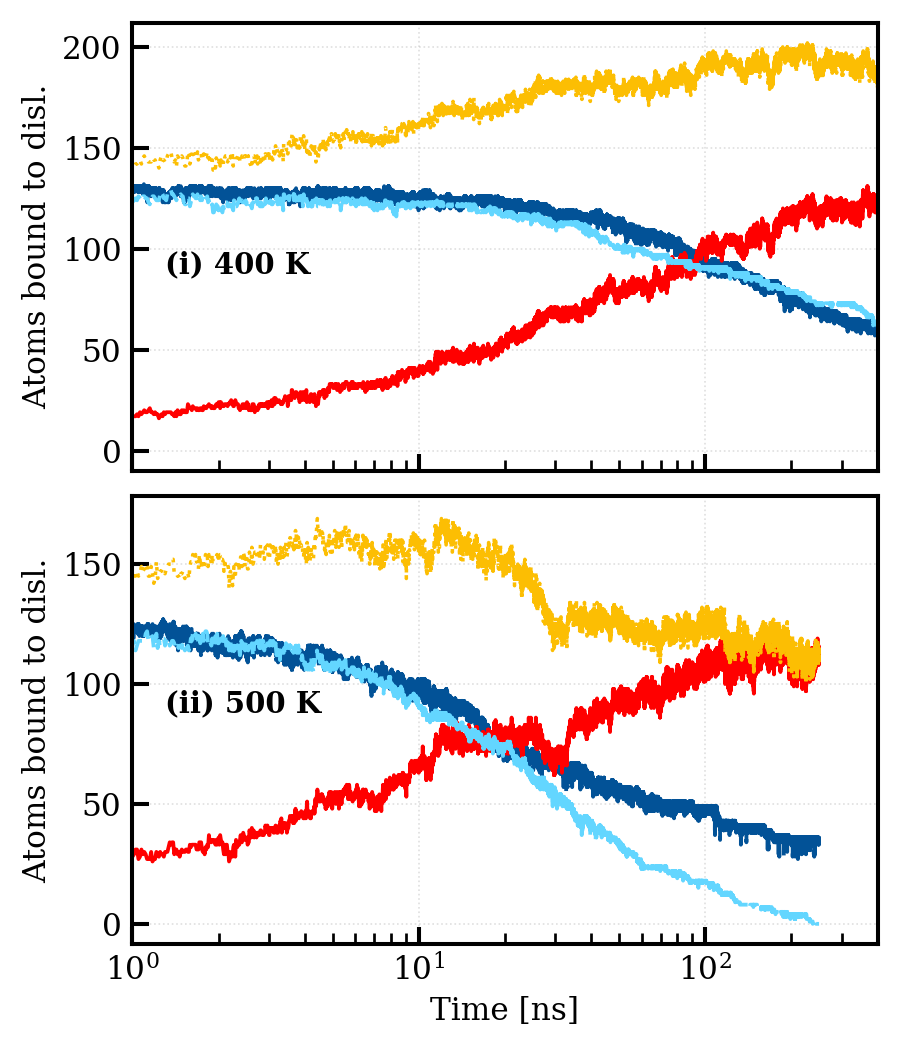
\includegraphics[width=0.99\textwidth]{disloc_isoEx_HT_log.png}  
  \caption{Logarithmic time scale}
  %\label{fig:sub-first}
\end{subfigure}
\begin{subfigure}{.5\textwidth}
  \centering
  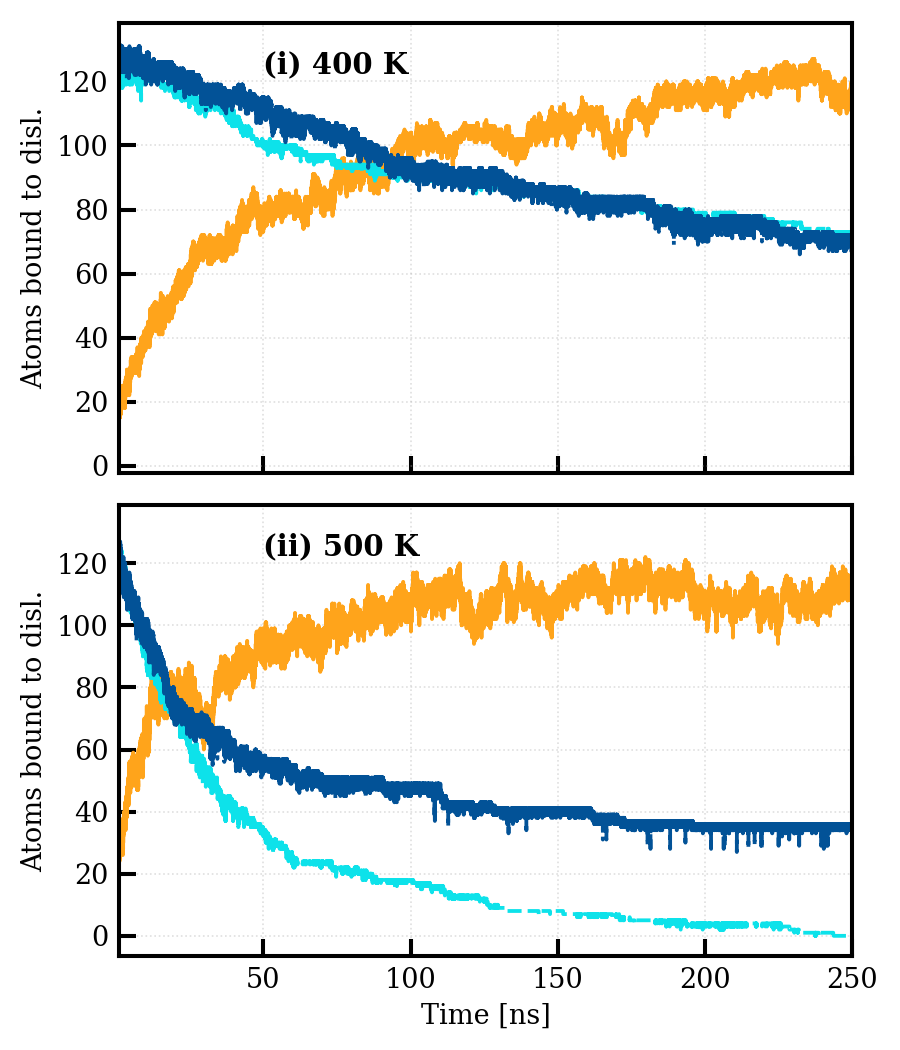
\includegraphics[width=0.99\textwidth]{disloc_isoEx_HT.png}  
  \caption{Linear time scale}
  %\label{fig:sub-second}
\end{subfigure}
   \caption{Number of H and T atoms bound to the dislocation for isotope exchange and diffusion simulations}
   \label{Fig:disloc_results} 
\end{figure}



% ----------------------------------------------------------------------------------
\section{Grain boundaries}
% ----------------------------------------------------------------------------------
The grain boundary results are shown in fig. \ref{Fig:GB_results}

\begin{figure}[ht]
\begin{subfigure}{.5\textwidth}
  \centering
 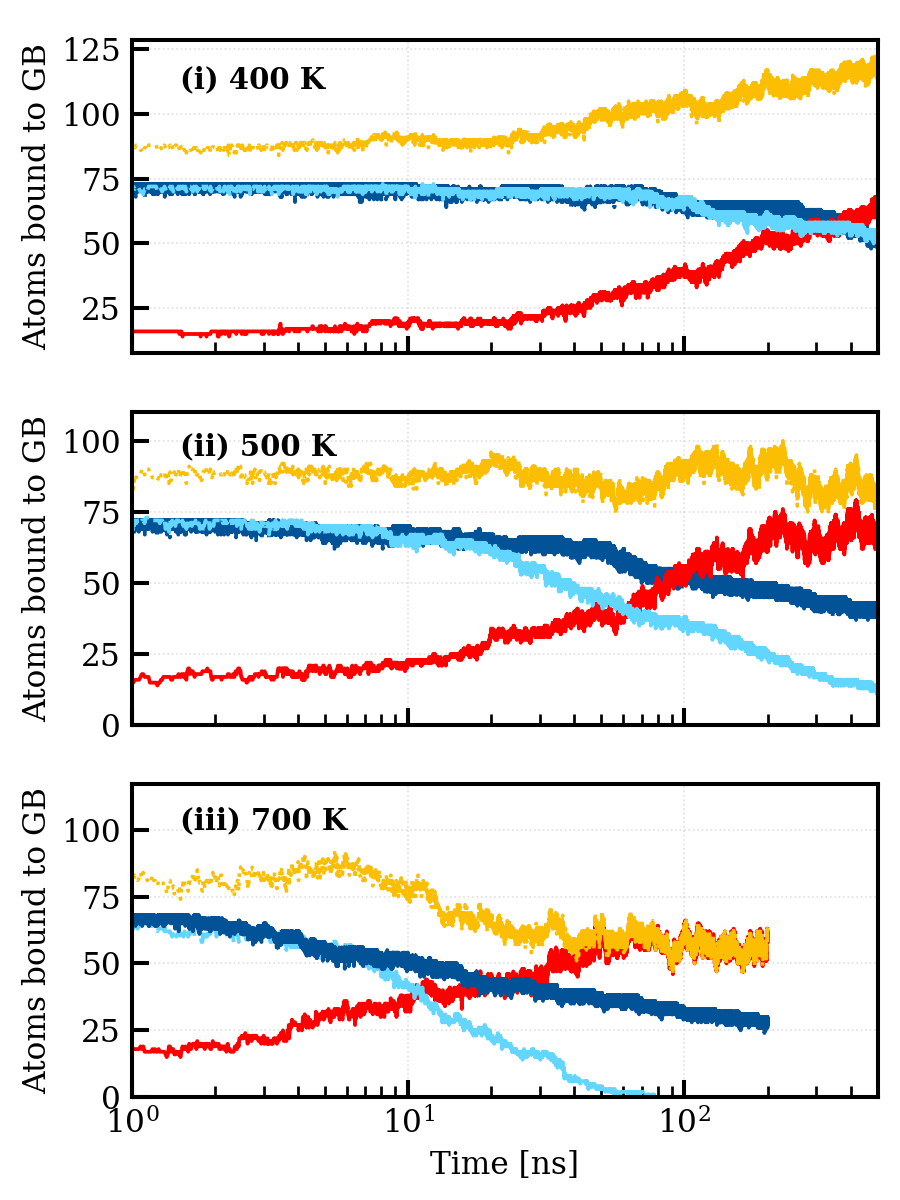
\includegraphics[width=0.99\textwidth]{GB_isoEx_HT_log.png}  
  \caption{Logarithmic time scale}
  %\label{fig:sub-first}
\end{subfigure}
\begin{subfigure}{.5\textwidth}
  \centering
  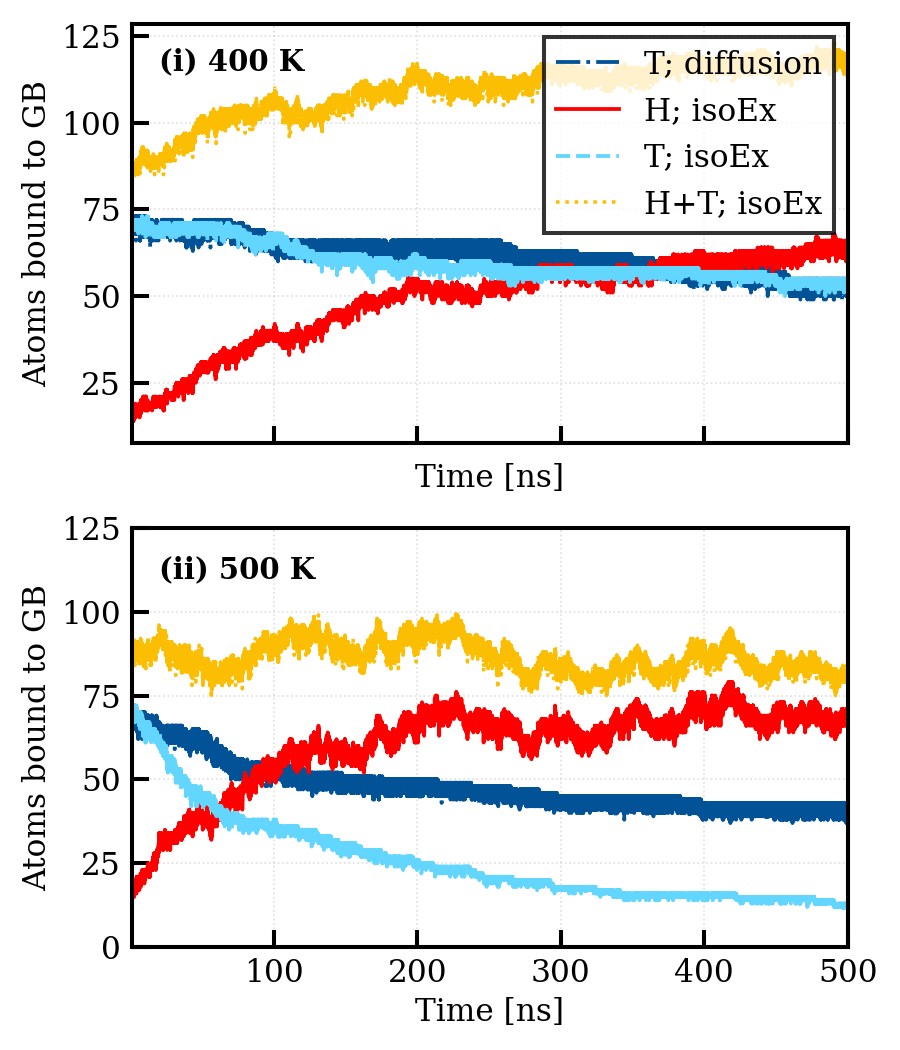
\includegraphics[width=0.99\textwidth]{GB_isoEx_HT.png}  
  \caption{Linear time scale}
  %\label{fig:sub-second}
\end{subfigure}
   \caption{Number of H and T atoms bound to the grain boundary for isotope exchange and diffusion simulations}
   \label{Fig:GB_results} 
\end{figure}

